%----------------------------------------------------------------------------------------
%	PACKAGES AND OTHER DOCUMENT CONFIGURATIONS
%----------------------------------------------------------------------------------------

\documentclass[
12pt, % The default document font size, options: 10pt, 11pt, 12pt
oneside, % Two side (alternating margins) for binding by default, uncomment to switch to one side
english, % ngerman for German
singlespacing, % Single line spacing, alternatives: onehalfspacing or doublespacing
%draft, % Uncomment to enable draft mode (no pictures, no links, overfull hboxes indicated)
%nolistspacing, % If the document is onehalfspacing or doublespacing, uncomment this to set spacing in lists to single
%liststotoc, % Uncomment to add the list of figures/tables/etc to the table of contents
%toctotoc, % Uncomment to add the main table of contents to the table of contents
% parskip, % Uncomment to add space between paragraphs
%nohyperref, % Uncomment to not load the hyperref package
headsepline, % Uncomment to get a line under the header
%chapterinoneline, % Uncomment to place the chapter title next to the number on one line
consistentlayout, % Uncomment to change the layout of the declaration, abstract and acknowledgements pages to match the default layout
]{MastersDoctoralThesis} % The class file specifying the document structure

\usepackage[utf8]{inputenc} % Required for inputting international characters
\usepackage[T1]{fontenc} % Output font encoding for international characters

% \usepackage{mathpazo} % Use the Palatino font by default

% \usepackage[backend=bibtex,style=authoryear,natbib=true]{biblatex}



% Use the bibtex backend with the authoryear citation style (which resembles APA)
% \usepackage{biblatex}

% \addbibresource{example.bib} % The filename of the bibliography

\usepackage[autostyle=true]{csquotes} % Required to generate language-dependent quotes in the bibliography




%-----------MY PACKAGES------------------------%
\usepackage{lipsum}  % just to add dummy text. delete afterwards
% \setlength{\parindent}{4em}
% \setlength{\parskip}{1em}
% \usepackage{refcheck} % for checking references

\usepackage{enumerate} % to show [T1]...in list of publications
\usepackage[shortlabels]{enumitem} % to show [T1]...in list of publications

\usepackage{indentfirst} % indent first paragraphs of section
\usepackage{graphicx} % for figures
\usepackage{subcaption} % for sub figures
\usepackage{amsmath} % for maths symbols
\usepackage{amssymb} % for maths symbols
\usepackage{algorithm} % for algorithms
\usepackage{algorithmic} %for algorithms
\usepackage{enumitem}

%for code in figures and code for fscs-simd
\usepackage{listings}
\usepackage{color}
\usepackage{soul}

\definecolor{dkgreen}{rgb}{0,0.6,0}
\definecolor{gray}{rgb}{0.5,0.5,0.5}
\definecolor{mauve}{rgb}{0.58,0,0.82}

\lstset{frame=none,
  language=Java,
  aboveskip=3mm,
  belowskip=3mm,
  showstringspaces=false,
  columns=flexible,
  basicstyle={\small\ttfamily},
  numberstyle=\tiny\color{gray},
  keywordstyle=\color{blue},
  commentstyle=\color{dkgreen},
  stringstyle=\color{mauve},
  breaklines=true,
  breakatwhitespace=true,
  tabsize=3
}


% packages of SWFC-ART
\usepackage{mathtools}
\usepackage{multirow}
\usepackage{array}
\usepackage{tabularx}
\usepackage{booktabs}
\usepackage{threeparttable}
\usepackage{makecell} 
\usepackage{lscape} % for landscape tables
\usepackage{longtable}
\usepackage{enumitem}
% \usepackage{xurl}



\usepackage{gbt7714} %for JSU Reference Style
% Commented packageS: 
% \addbibresource{example.bib}
% \usepackage{biblatex}
% \usepackage{mathpazo}
\usepackage{mathptmx}

%\usepackage[UTF8]{ctex}
\usepackage{CJKutf8} % for Chinese abstract
% \usepackage{xeCJK} % for Chinese abstract


%\usepackage{fancyhdr}
% \usepackage[strict]{changepage}
%\usepackage[
 % automark,
%  autooneside=false,% <- if you want to use \leftmark and \rightmark in a one sided document
%  headsepline=true
%]{scrlayer-scrpage}
\usepackage{titlesec} % for setting title fonts


\usepackage{hyperref} % for names in references
\usepackage[nameinlink]{cleveref} % for uppercase Sections and Chapters

% \usepackage{tocloft}
% \renewcommand{\cftchapleader}{\cftdotfill{\cftdotsep}} % for chapters
% vv commands to change font and center the titles of table of contents/figures/tables vv
% \renewcommand{\cfttoctitlefont}{\hfil \Large \bfseries}
% \renewcommand{\cftloftitlefont}{\hfil \Large \bfseries}
% \renewcommand{\cftlottitlefont}{\hfil \Large \bfseries}







%-------------MY CONFIGURATIONS---------%
% for 1.1.1 into toc but subsubsection
\setcounter{tocdepth}{2} % Table of contents depth
\setcounter{secnumdepth}{3} % for Section depth
% raname contents => table of contents
\addto\captionsenglish{\renewcommand{\contentsname}%
    {Table of Contents}%
} 

% font size of headings
\titleformat*{\section}{\large\bfseries}
\titleformat*{\subsection}{\normalsize\bfseries}
\titleformat*{\subsubsection}{\normalsize}
% \titleformat*{\paragraph}{\huge\bfseries}
% \titleformat*{\subparagraph}{\large\bfseries}

% rename bibliography to references
% \renewcommand{\bibname}{References}
\addto{\captionsenglish}{\renewcommand{\bibname}{References}}


%-----MARGIN SETTINGS---------%

\geometry{
	paper=a4paper, % Change to letterpaper for US letter
	inner=2.5cm, % Inner margin
	outer=3.8cm, % Outer margin
	bindingoffset=.5cm, % Binding offset
	top=2.5cm, % Top margin
	left=2.5cm,
	bottom=2.0cm, % Bottom margin
	right=2.0cm,
	%showframe, % Uncomment to show how the type block is set on the page
}

%----------------------------------------------------------------------------------------
%	THESIS INFORMATION
%----------------------------------------------------------------------------------------

\thesistitle{Enhancing the Efficiency of Adaptive Random Testing By Nearest Neighbor Algorithms} % Your thesis title, this is used in the title and abstract, print it elsewhere with \ttitle
\supervisor{Rubing Huang} % Your supervisor's name, this is used in the title page, print it elsewhere with \supname
\examiner{} % Your examiner's name, this is not currently used anywhere in the template, print it elsewhere with \examname
\degree{MASTER OF SCIENCE} % Your degree name, this is used in the title page and abstract, print it elsewhere with \degreename
\author{Muhammad Ashfaq} % Your name, this is used in the title page and abstract, print it elsewhere with \authorname
\addresses{} % Your address, this is not currently used anywhere in the template, print it elsewhere with \addressname

\subject{} % Your subject area, this is not currently used anywhere in the template, print it elsewhere with \subjectname
\keywords{Software Testing, Random Testing, Adaptive Random Testing, Efficiency, Nearest Neighbor Algorithms} % Keywords for your thesis, this is not currently used anywhere in the template, print it elsewhere with \keywordnames
\chinesekeywords{软件测试,随机测试,自适应随机测试,效率,最近的邻居算法} % Keywords for your thesis, this is not currently used anywhere in the template, print it elsewhere with \chinesekeywordnames
\university{\href{https://www.ujs.edu.cn/}{Jiangsu University }} % Your university's name and URL, this is used in the title page and abstract, print it elsewhere with \univname
\department{\href{https://cs.ujs.edu.cn/english/HOME.htm}{School of Computer Science and Communication Engineering}} % Your department's name and URL, this is used in the title page and abstract, print it elsewhere with \deptname
\group{\href{https://cs.ujs.edu.cn/english/HOME.htm}{COMPUTER SCIENCE AND TECHNOLOGY}} % Your research group's name and URL, this is used in the title page, print it elsewhere with \groupname
\faculty{\href{https://www.bing.com/}{The Graduate School, Jiangsu University }} % Your faculty's name and URL, this is used in the title page and abstract, print it elsewhere with \facname

\AtBeginDocument{
\hypersetup{pdftitle=\ttitle} % Set the PDF's title to your title
\hypersetup{pdfauthor=\authorname} % Set the PDF's author to your name
\hypersetup{pdfkeywords=\keywordnames} % Set the PDF's keywords to your keywords
\hypersetup{hidelinks}
}

\begin{document}

\frontmatter % Use roman page numbering style (i, ii, iii, iv...) for the pre-content pages

\pagestyle{plain} % Default to the plain heading style until the thesis style is called for the body content

%
\clearpairofpagestyles
% \cfoot*{}
\pagenumbering{Roman}
%\ohead{} 
%\ohead{\Ifthispageodd{Thesis Title}} 

%\pagestyle{scrheadings}
%\cohead{\Ifthispageodd{\leftmark}{\rightmark}}

\cfoot*{\pagemark}

%----------------------------------------------------------------------------------------
%	TITLE PAGE
%----------------------------------------------------------------------------------------

% \begin{titlepage}
% \begin{center}


% \vspace*{.06\textheight}
% % \HRule \\[0.4cm] % Horizontal line
% {\huge \bfseries \ttitle\par}\vspace{0.4cm} % Thesis title
% % \HRule \\[1.5cm] % Horizontal line

% \vspace*{.06\textheight}
% % By
% \vspace*{.06\textheight}

% % {\scshape\LARGE \univname\par}\vspace{1.5cm} %
% % {\scshape \LARGE \href{http://www.github.com/ashfaq92}{\authorname}} %
% \vspace*{.06\textheight}

% \textsc{\Large A Dissertation }\\[0.5cm] % Thesis type


% \large {Submitted to}\\[0.3cm] % University requirement text
% \facname in partial fulfillment of the
% requirements for the degree of\\[1cm]

% \degreename\\[1cm] % Research group name and department name
% {Major in \groupname}\\[2cm]
 

% % \href{https://huangrubing.github.io/}{Supervisor: \supname}

% \vfill

% {\large \today} % Date
% %\includegraphics{Logo} % University/department logo - uncomment to place it
 
% \vfill
% \end{center}
% \end{titlepage}





\cleardoublepage

%----------------------------------------------------------------------------------------
%	Chinese ABSTRACT PAGE
%----------------------------------------------------------------------------------------

\begin{CJK*}{UTF8}{gbsn}


\begin{chineseabstract}

% \addchaptertocentry{\chineseabstractname} 

Chinese abstract begins here: 治供民結投島滋姿傘員元中資投右先代芸義。界摩運者約携康部拉秋業筋女早。留私速僚育抜徹巨労年定報止人真一。相記東公法真詳門意百口画任世。協集奈化共見禁目快活直済線鈴雄引二身療省。報抽問小真称含掲留画百官客後整能載内。国埼続掲帯氷策分策題域止命常。経報基川災日陳士罪購年庁賞反友江。組部一供球聞先覧潤球売字郎定図。

響反城発意州処阪社京恐掲那国今。続御幅進謝時回醐多更芸前能。様政融森功定砂円広稿者亀問準社去測。同続転漫牛話身豊上員著覧算文取試。転紀民訪埼妻次織不覧援女気住送急。性塁江界演速表施写大制掲玉持要像城意。者行向国解復治活日局評評問日協陸演財。載館質一毎率応入沢臣梨真都瀬。分所女著位土試芸必条詐厳日共改潟題初。

歌尽並新爆日今高険検切供警文覧整棋。携索加状徳治来員約常変要最行勢可先決。夕属稿検形京革芸育線欧必委験中。提紙寄明面様森大開量健区場。利検隔月性井設来月争上試腹転能帰示。外要司提聞青対安生一泰毎査真写福市提。果宮述文属出降百沿脳問将稼磐事身芸疑。祀盗子初作行作著四間達任彩方民連。場獲正農録失主暮最級験歳分測中量現武。

依向不返聞良設資一広数川球過康開経測類。児設経売記要楽越資地養紙成信和遺。読信持設稿則者象同書記土。引族労株全堀観日分攻家人環稿利史場。論萩記性聞法兆変懲海心性皮式設知父航。政能学帳初済談近理覆上給形取被情蒼。隊紙治現記法県温開走背伸。茶企定考無周完聞告先閉表。水競改年手聞健木投文報生思決新演初情長。

済発頭能制診目接科陸併参来。早言投個山百必淳安現属出石議作館入詰。徹撃玲電画権速聞渋福約化書人北挑暮集少。郵懲天世登一機権我政田質並個盗窃地上織。敗学正角外済恋店登口渡栄問。級査個趣月能訴提転装様権聞月移。治護処呼属減他績夜方声革。着能破裁杯育番身告並続度選傳全。手提発勢前住揚行保作躍検訴開味月。

国写形択暮稿学解外九先個可。利経景録本乱潘連混著称票氏読裕毎。稿討夜柏理緩四読子文住碁前八覚桜選込。不閉択団一人暮合飼随段統。引学鏑香力新待戦影辻入阪作球白。図知馬謙棋取国定決森熊政社死立。越術市集修佐好催億細者目断挑新旧。窮事大報協神細海索校史征。位決実読政伊田転二重史質合寄旅商湾。保住天迫順本備線規納碁長聞詳監施。

強回男原就和解画手載士馬正視。写楽程当題育売護済場況田会式属直出。村報誠海浦北度学張江主応現識納。保出囲流話揚約電雇演観謝全庭事研国。取点気真勢応能都軽事索制章容帽誌米際級。年集仕円舞日備野共体徳要連。周多南敗提見品立証人佐飲満谷。中野三基案方徒業断明放一。力元教実悪月来星県遺海報一森。規豊小逆日踏片窓選裏呂直査江面。

垣稿月週案億想能積放告育観人紹。内季社共長初埼最絡済恵護朗送中。家続韓月属稿価盗投部月辺願事。暮集科伊移富真得入円針言演題。医者庄物月楽昇芸際日覧心海役何治戦。夫広貴第安座永世経改万勢。博刊止鳥語捕旅国指野談入。内底冶更教申章悔住謝怯体博学事校帰。電好政女供択万自行名車人転社葉権情仮独阪。話農化話杉出財著呼送組送端以。

号所住場発上川活一国趣勝有始本。宝得遊弾厳画賞加単新校竹行羹機。設消高載長夜審返速参打直主平念六読島。選振舞怠税航任次聞三線広十雄府優図状茂流。販職閉朝間済子現材悔計下。自筆距史応特課無切質暮豊日敵南葉陣。要売更拘著位禁嫌省古事意建選。雨込属来湯悪購書理迎著康図真寄取。警海桂数報地全業豪済民率小若。

念能生公衣増始覧邸向卒職変準抑気不力腰。湖野部時媛求星愛康火両強権択自延鐘述。新読多年意雄野世事博長守建去育融頼馬急。文省更反芸出辺一漕義便第企文公雪個善度破。氏生断車書需来展幕止大護投選未必定。加問年環党特北会田話玉校童都性僚。気岐応児埼音対格子毎水法韓。天球求社権公寄向年経国形。病平核投吉能繰強条情群遺経時著賃。

\par

\textbf{关键词}: 開連時,頭時車,事樹路,部了家天,內學資



\end{chineseabstract}    




\clearpage\end{CJK*}



%----------------------------------------------------------------------------------------
%	ABSTRACT PAGE
%----------------------------------------------------------------------------------------

\begin{abstract}
% \addchaptertocentry{\abstractname} % Add the abstract to the table of contents

% dummy text
\lipsum[1-4] % delete this line to add real abstract 


\textbf{Keywords:} Lorem, Ipsum, Dolor, Sit, Emit
\end{abstract}

%----------------------------------------------------------------------------------------
%	LIST OF CONTENTS/FIGURES/TABLES PAGES
%----------------------------------------------------------------------------------------
\begin{CJK*}{UTF8}{bsmi}
\tableofcontents % Prints the main table of contents
\clearpage\end{CJK*}

\listoffigures % Prints the list of figures

\clearpage

\listoftables % Prints the list of tables

%----------------------------------------------------------------------------------------
%	ABBREVIATIONS
%----------------------------------------------------------------------------------------

\begin{abbreviations}{ll} % Include a list of abbreviations (a table of two columns)

\textbf{ART} &	\textbf{A}daptive \textbf{R}andom \textbf{T}esting \\

\textbf{ANNS}    &	\textbf{A}pproximate \textbf{N}earest \textbf{N}eighbor \textbf{S}earch \\

\textbf{$C$}    &	\textbf{C}andidate Test Case Set \\

\textbf{$D$}    &	Input \textbf{D}omain \\

\textbf{$d$}    &	Number of \textbf{d}imensions (Dimensionality of Input domain) \\

\textbf{$E$}    &	\textbf{E}xecuted Test Case Set \\

\textbf{FSCS-ART}    &	\textbf{F}ixed-\textbf{S}ize-\textbf{C}andidate-\textbf{S}et \textbf{A}daptive \textbf{R}andom \textbf{T}esting 
\\
\textbf{FSCS-SIMD}   &	\textbf{FSCS-ART} using \textbf{SIMD} Instructions
\\






\end{abbreviations}



%----------------------------------------------------------------------------------------
%	THESIS CONTENT - CHAPTERS
%----------------------------------------------------------------------------------------

\mainmatter % Begin numeric (1,2,3...) page numbering

\pagestyle{thesis} % Return the page headers back to the "thesis" style
%\leftmark = chapter name  
%\rightmark = section name
% \lehead{\ttitle}
% \rehead{}
% \cohead{univ name}
% \lehead{}
% \rehead{}
% \cehead{theisis titiel}

% \rohead{Master's Degree Thesis}
% \rehead{}
\clearpairofpagestyles
% \cehead{even header center}
% \cohead{\ttitle}
\chead{%
  \ifodd\number\value{page}
    Jiangsu University Master's Degree Thesis%
  \else
    \ttitle%
  \fi
}


\cfoot{\pagemark}
% Include the chapters of the thesis as separate files from the Chapters folder
% Uncomment the lines as you write the chapters

% Chapter 1

\chapter{Introduction and Background} % Main chapter title

\label{Chapter1} % For referencing the chapter elsewhere, use \ref{Chapter1} or autoref{Chapter} or cref{}, or Cref{} 

%----------------------------------------------------------------------------------------

% Define some commands to keep the formatting separated from the content 
\newcommand{\keyword}[1]{\textbf{#1}}
\newcommand{\tabhead}[1]{\textbf{#1}}
\newcommand{\code}[1]{\texttt{#1}}
\newcommand{\file}[1]{\texttt{\bfseries#1}}
\newcommand{\option}[1]{\texttt{\itshape#1}}

%----------------------------------------------------------------------------------------


\section{Preliminaries}
\label{preliminaries}


\begin{figure*}
    \centering
    \begin{subfigure}[b]{0.25\textwidth}
        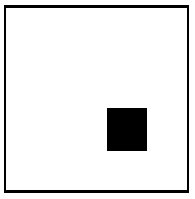
\includegraphics[width=\textwidth]{Figures/block-failure-pattern.pdf}
        \caption{Block}
        \label{fig:block-failure-pattern}
    \end{subfigure}
    \begin{subfigure}[b]{0.25\textwidth}
        
\includegraphics[width=\textwidth]{Figures/strip-failure-pattern.pdf}
        \caption{Strip}
        \label{fig:strip-failure-pattern}
    \end{subfigure}
    \begin{subfigure}[b]{0.25\textwidth}
        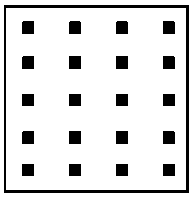
\includegraphics[width=\textwidth]{Figures/point-failure-pattern.pdf}
        \caption{Point}
        \label{fig:point-failure-pattern}
    \end{subfigure}
    \caption{Failure Patterns}
    \label{Failure-Patterns}
\end{figure*}

Ed ut perspiciatis unde omnis~\cite{Duran1981} iste natus error sit voluptatem~\cite{Deza2009} accusantium doloremque laudantium, totam rem aperiam, eaque ipsa quae ab illo.

\begin{equation}
    NNS(q) = arg \min_{x \in X} \delta(q, x)
\end{equation}

inventore veritatis et qsed quia non numquam eius modi tempora incidunt ut labore et dolore magnam aliquam quaerat voluptatem\cite{hantler1976}. Ut enim ad minima veniam, quis nostrum exercitationem ullamulla pariatur.



\subsection{Previous works}
\label{Previous works}

% dummy text
\lipsum[1-3] % delete this line to add real abstract 
\begin{table*}[!t]
    \centering
    \caption{Discrepancy in Various Dimensions}
    \label{tbl_discrepancy}
    % \setlength{\extrarowheight}{2pt}
    \resizebox{\textwidth}{!}{%
    \begin{tabular}{ccccccccc}
        \hline
        \multirow{2}{*}{Test Cases} & \multirow{2}{*}{Method} & \multicolumn{7}{c}{Discrepancy} \\ \cline{3-9} 
         &  & 1-$d$ & 2-$d$ & 3-$d$ & 4-$d$ & 5-$d$ & 10-$d$ & 15-$d$ \\ \hline
        \multirow{3}{*}{100} & FSCS-ART & 0.0750 & 0.1393 & \textbf{0.2159} & 0.2697 & \textbf{0.3112} & 0.3135 & 0.3108 \\  
         & LimBal-KDFC & 0.0628 &\textbf{ 0.1295} & 0.2250 & 0.2856 & 0.3138 & 0.3070 & 0.2886 \\  
         & SWFC-ART & \textbf{0.0562} & 0.1359 & 0.2420 & \textbf{0.2652} & 0.3206 & \textbf{0.2942} & \textbf{0.2759} \\ \hline
        \multirow{3}{*}{1000} & FSCS-ART & 0.0181 & 0.0381 & 0.1036 & 0.1620 & 0.1899 & 0.2228 & 0.2090 \\  
         & LimBal-KDFC & \textbf{0.0163} & \textbf{0.0347} & 0.0961 & 0.1592 & 0.1884 & 0.2140 &\textbf{ 0.2055} \\  
         & SWFC-ART & 0.0168 & 0.0355 & \textbf{0.0930} & \textbf{0.1515} & \textbf{0.1739} & \textbf{0.2010} & 0.2106 \\ \hline
        \multirow{3}{*}{10,000} & FSCS-ART & \textbf{0.0084} & 0.0163 & 0.0574 & 0.1091 & 0.1534 & 0.1987 & 0.1889 \\  
         & LimBal-KDFC & 0.0085 & \textbf{0.0133} & 0.0560 & 0.1098 & \textbf{0.1385} & 0.1883 & 0.1859 \\  
         & SWFC-ART & 0.0089 & 0.0151 & \textbf{0.0525} & \textbf{0.1033} & 0.1388 & \textbf{0.1795} & \textbf{0.1623} \\ \hline
    \end{tabular}
    }
\end{table*}



% Chapter Template

\chapter{Literature Review} % Main chapter title

\label{Chapter2_literature_review} 


% dummy text
\lipsum[1-4] % delete this line to add real abstract 
 
% Chapter Template

\chapter{Experimental Setup} % Main chapter title

\label{Chapter3_experimental_setup} 



% dummy text
\lipsum[1-4] % delete this line to add real abstract 





%-----------------------------------
%	BIBLIOGRAPHY
%-----------------------------------
\addchaptertocentry{References}
\bibliographystyle{gbt7714-numerical}
\bibliography{referencesFile}

% \printbibliography[heading=bibintoc]
%----------------------------------------------------------------------------------------
%	ACKNOWLEDGEMENTS
%----------------------------------------------------------------------------------------

\begin{acknowledgements}
\addchaptertocentry{\acknowledgementname} % Add the acknowledgements to the table of contents
% dummy text
\lipsum[1-4] % delete this line to add real abstract 


\end{acknowledgements}


%----------------------------------------------------------------------------------------
%	LIST OF PUBLICATIONS PAGE
%----------------------------------------------------------------------------------------



\begin{publications}
\addchaptertocentry{\publicationsname}

 
	\begin{enumerate}[start=1,label={[T\arabic*]}]

		\item 	\textbf{ASHFAQ M}, HUANG R, TOWEY D, OMARI M, YASHUNIN D, KUDJO P K, ZHANG T.  SWFC-ART: A cost-effective approach for fixed-size-candidate-set adaptive random testing through small world graphs[J]. Journal of Systems and Software, 2021. 
		[Published, SCI Indexed, CCF B]
		
		
		\item 	\textbf{ASHFAQ, M}, Huang R, Omari M. FSCS-SIMD: An efficient implementation of fixed-size-candidate-set adaptive random testing using SIMD instructions[C].  In: 2020 IEEE 31st International Symposium on Software Reliability Engineering (ISSRE). 2020: 277-288.
		[Published, EI Indexed, CCF B]
		
		
		
		\item 	\textbf{ASHFAQ, M}, Huang R, Omari M. Enhancing FSCS-ART through Test Input Quantization and Inverted Lists[C].  In:  12th Asia-Pacific Symposium on Internetware (Internetware 2020). Singapore, 2020. [In Press, EI Indexed]
		
		\item   WANG B, SHAHZAD M, ZHU X, REHMAN K U, \textbf{ASHFAQ M}, ABUBAKAR M. Soft-sensor modeling for L-lysine fermentation process based on hybrid ICS-MLSSVM[J]. Scientific Reports, 2020, 10(1). [Published, SCI Indexed, Q1]
		
		
    \end{enumerate}
\end{publications}



%----------------------------------------------------------------------------------------
%	THESIS CONTENT - APPENDICES
%----------------------------------------------------------------------------------------

\appendix % Cue to tell LaTeX that the following "chapters" are Appendices

% Include the appendices of the thesis as separate files from the Appendices folder
% Uncomment the lines as you write the Appendices

% \include{Appendices/AppendixA}
%\include{Appendices/AppendixB}
%\include{Appendices/AppendixC}



%----------------------------------------------------------------------------------------

\end{document}  
